\documentclass[12pt,a4paper]{article}

\usepackage{fancyhdr}
\usepackage{titling}

\usepackage[a4paper,margin=1in]{geometry}
\usepackage[hidelinks]{hyperref}
\hypersetup{
    colorlinks=true,
    linkcolor=blue,
    filecolor=magenta,
    urlcolor=blue,
    citecolor=blue,
    pdftitle={Deep Learning Homework 7 Report},
    pdfauthor={Cheng-Liang Chi},
}
\usepackage{xspace}
\usepackage[svgnames]{xcolor}
\usepackage[outputdir=build]{minted}
\definecolor{bgcolor}{rgb}{0.95, 0.95, 0.95}  % Light gray background for readability
\setminted{
    fontsize=\small,    % Adjust code font size
    linenos=true,       % Enable line numbers
    numbersep=5pt,      % Space between numbers and code
    frame=single,       % Box around code
    framesep=2mm,       % Padding inside the frame
    bgcolor=bgcolor,    % Background color
    breaklines=true,    % Line breaking
    tabsize=4           % Consistent tab width
}

\usepackage[T1]{fontenc}
\usepackage{inconsolata}
\usepackage{newtxtext,newtxmath}
\usepackage[expanded]{mfirstuc}

\usepackage{graphicx}
\usepackage{caption}
\usepackage{subcaption}
\usepackage{animate}

\usepackage{pgfplots}
\usepackage{pgfplotstable}
\usetikzlibrary{plotmarks}
\usepgfplotslibrary{groupplots}
\pgfplotsset{compat=1.18}

\usepackage{amsmath}
\usepackage{multirow}
\usepackage{booktabs}
\usepackage{array}
\usepackage{diagbox}

\usepackage[
    backend=biber,
    style=ieee,
    sortcites=true,
]{biblatex}
\addbibresource{references.bib}

\title{Deep Learning Homework 7 Report}
\author{Cheng-Liang Chi}
\date{\today}

\begin{document}
\maketitle

\pagestyle{fancy}
\fancyhead[L]{\thetitle}
\fancyhead[R]{\theauthor}

\tableofcontents
\newpage
\newcommand{\pendulum}{\href{https://www.gymlibrary.dev/environments/classic_control/pendulum/}{\texttt{Pendulum-v1}}\xspace}
\newcommand{\walker}{\href{https://www.gymlibrary.dev/environments/mujoco/walker2d/}{\texttt{Walker2d-v4}}\xspace}

\section{Introduction}
\label{sec:introduction}

This report details the implementation and analysis of two prominent policy-based reinforcement learning methods: Advantage Actor-Critic (A2C)~\cite{han2020actorcriticreinforcementlearningcontrol} and Proximal Policy Optimization (PPO)~\cite{schulman2017proximal}, specifically employing PPO-Clip~\cite{huang2024ppoclipattainsglobaloptimality} with Generalized Advantage Estimation (GAE)~\cite{schulman2018highdimensionalcontinuouscontrolusing}.
Utilizing PyTorch~\cite{PyTorch2} and OpenAI Gym~\cite{brockman2016openai} environments, this work systematically explores and evaluates these methods on the \pendulum environment as well as a more challenging MuJoCo~\cite{MuJoCo} locomotion task, \walker.

The objective of this assignment is to:

Develop a thorough understanding of the key components and algorithms underlying policy-based reinforcement learning approaches.

Gain practical experience by implementing and optimizing A2C~\cite{han2020actorcriticreinforcementlearningcontrol} and PPO~\cite{schulman2017proximal} algorithms with GAE~\cite{schulman2018highdimensionalcontinuouscontrolusing} in PyTorch~\cite{PyTorch2}.

Analyze and compare the performance, training stability, and sample efficiency of A2C versus PPO through empirical experimentation.

The report is organized into several key sections:
Section \ref{sec:implementation} describes the specifics of the implemented algorithms, including methods used to obtain stochastic policy gradients, advantage estimations, and sample collections.
Section \ref{sec:discussion} presents experimental results, with detailed comparisons between A2C and PPO implementations.

\section{Implementation Details}
\label{sec:implementation}

\section{Discussion}

\subsection{Default Configuration}

The results of the default configuration are shows in Figure \ref{fig:default}.
The default configuration is using four down and up-blocks, and keep the attention layers only at the lowest resolution (bottom) layers to reduce memory usage.
And the model is trained for 300 epochs with a batch size of 32 and time steps of 1000.

\begin{figure}[H]
    \centering
    \begin{subfigure}{0.48\textwidth}
        \centering
        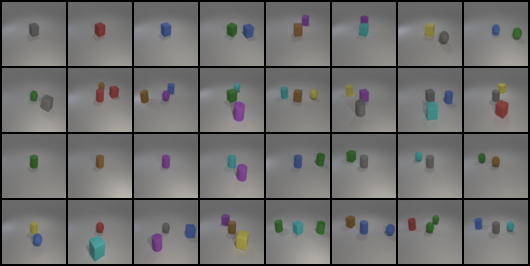
\includegraphics[width=\textwidth]{figures/default_test.png}
        \caption{Default Configuration Results on Test Set with accuracy of 0.9479}
        \label{fig:default_test}
    \end{subfigure}
    \hfill
    \begin{subfigure}{0.48\textwidth}
        \centering
        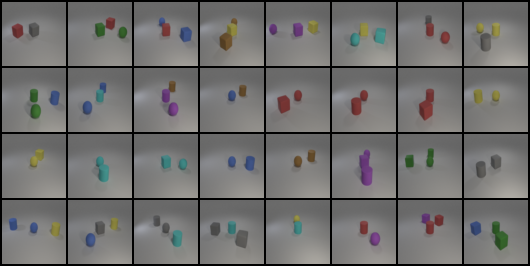
\includegraphics[width=\textwidth]{figures/default_new_test.png}
        \caption{Default Configuration Results on New Test Set with accuracy of 0.9271}
        \label{fig:default_new_test}
    \end{subfigure}
    \caption{Default Configuration Results and Accuracy}
    \label{fig:default}
\end{figure}

And the results of the manual test with ``red sphere'', ``cyan cylinder'', and ``cyan cube'' are shown in Figure \ref{fig:default_manual}.
\begin{figure}[H]
    \centering
    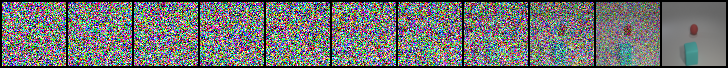
\includegraphics[width=\textwidth]{figures/default_manual_test.png}
    \caption{Default Configuration Results on Manual Test Set with accuracy of 1.0000}
    \label{fig:default_manual}
\end{figure}

And the loss curve of the default configuration is shown in Figure \ref{fig:loss_curve}.

\subsection{Same model with different time steps}

\subsubsection{500 Time Steps}
The results of the same model with different time steps are shown in Figure \ref{fig:step_500}.
The model is trained for 300 epochs with a batch size of 32 and time steps of 500.
\begin{figure}[H]
    \centering
    \begin{subfigure}{0.48\textwidth}
        \centering
        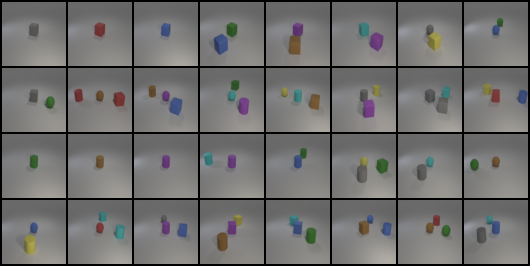
\includegraphics[width=\textwidth]{figures/step_500_test.png}
        \caption{500 Time Steps Results on Test Set with accuracy of 0.9740}
        \label{fig:step_500_test}
    \end{subfigure}
    \hfill
    \begin{subfigure}{0.48\textwidth}
        \centering
        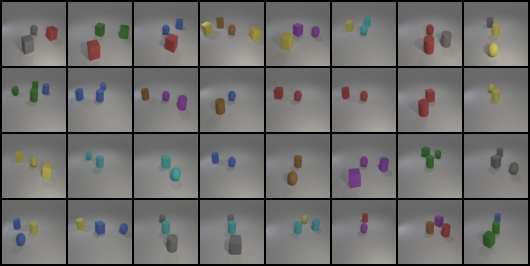
\includegraphics[width=\textwidth]{figures/step_500_new_test.png}
        \caption{500 Time Steps Results on New Test Set with accuracy of 0.8906}
        \label{fig:step_500_new_test}
    \end{subfigure}
    \caption{500 Time Steps Results and Accuracy}
    \label{fig:step_500}
\end{figure}

And the results of the manual test with ``red sphere'', ``cyan cylinder'', and ``cyan cube'' are shown in Figure \ref{fig:step_500_manual}.

\begin{figure}[H]
    \centering
    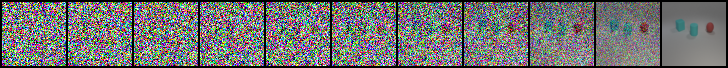
\includegraphics[width=\textwidth]{figures/step_500_manual_test.png}
    \caption{500 Time Steps Results on Manual Test Set with accuracy of 1.0000}
    \label{fig:step_500_manual}
\end{figure}
And the loss curve of the 500 time steps is shown in Figure \ref{fig:loss_curve}.

\subsubsection{100 Time Steps}

The results of the same model with different time steps are shown in Figure \ref{fig:step_100}.
The model is trained for 300 epochs with a batch size of 32 and time steps of 100.

\begin{figure}[H]
    \centering
    \begin{subfigure}{0.48\textwidth}
        \centering
        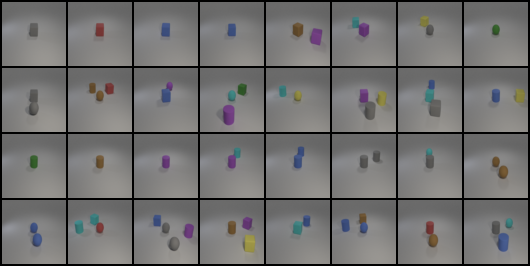
\includegraphics[width=\textwidth]{figures/step_100_test.png}
        \caption{100 Time Steps Results on Test Set with accuracy of 0.8021}
        \label{fig:step_100_test}
    \end{subfigure}
    \hfill
    \begin{subfigure}{0.48\textwidth}
        \centering
        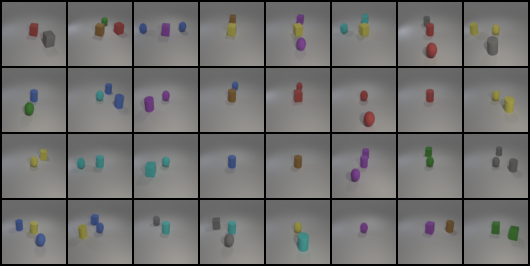
\includegraphics[width=\textwidth]{figures/step_100_new_test.png}
        \caption{100 Time Steps Results on New Test Set with accuracy of 0.7865}
        \label{fig:step_100_new_test}
    \end{subfigure}
    \caption{100 Time Steps Results and Accuracy}
    \label{fig:step_100}
\end{figure}

And the results of the manual test with ``red sphere'', ``cyan cylinder'', and ``cyan cube'' are shown in Figure \ref{fig:step_100_manual}.
\begin{figure}[H]
    \centering
    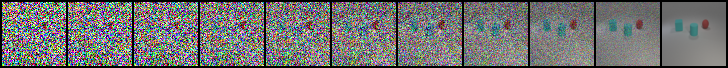
\includegraphics[width=\textwidth]{figures/step_100_manual_test.png}
    \caption{100 Time Steps Results on Manual Test Set with accuracy of 1.0000}
    \label{fig:step_100_manual}
\end{figure}

And the loss curve of the 100 time steps is shown in Figure \ref{fig:loss_curve}.

\subsection{Discussion of Results}

The results of the default configuration and the same model with different time steps are shown in Figure \ref{fig:loss_curve}.
The model with 1000 time steps has the lowest loss, and the model with 500 or 100 time steps has a higher loss.
We can see that the more time steps we have, the lower the loss is.


\begin{figure}[H]
    \begin{tikzpicture}
        \begin{axis}[
                title={Loss Curve of Default Configuration},
                xlabel={Epoch},
                xmin=0,
                xmax=300,
                ymode=log,
                ylabel={Loss},
                grid=major,
                width=\textwidth,
                height=0.5\textwidth,
                cycle list name=color list,
            ]
            \addplot table[col sep=comma, x=Step, y=Value] {csvs/default.csv};
            \addlegendentry{Train Loss with 1000 Time Steps}
            \addplot table[col sep=comma, x=Step, y=Value] {csvs/step-500.csv};
            \addlegendentry{Train Loss with 500 Time Steps}
            \addplot table[col sep=comma, x=Step, y=Value] {csvs/step-100.csv};
            \addlegendentry{Train Loss with 100 Time Steps}
            \addplot table[col sep=comma, x=Step, y=Value] {csvs/large.csv};
            \addlegendentry{Train Loss with 1000 Time Steps (Large Model)}
        \end{axis}
    \end{tikzpicture}
    \caption{Loss Curve of Different Time Steps}
    \label{fig:loss_curve}
\end{figure}

\subsection{Larger Model}

I also tried to use 6 down and up-blocks, and keep the attention layers only at the lowest two resolution (bottom) layers to reduce memory usage.
The model is trained for 300 epochs with a batch size of 32 and time steps of 1000.

Since the results shows similar with the previous model, I didn't include the results here.
But I will include the loss curve of the larger model.
The loss curve is shown in Figure \ref{fig:loss_curve_large}.



\printbibliography

\end{document}
